\documentclass[a4paper]{article}

%% Language and font encodings
\usepackage[english]{babel}
\usepackage[utf8x]{inputenc}
\usepackage[T1]{fontenc}

%% Sets page size and margins
\usepackage[a4paper,top=3cm,bottom=2cm,left=3cm,right=3cm,marginparwidth=2cm]{geometry}

%% Useful packages
\usepackage{algorithm}
\usepackage{amsfonts}
\usepackage{amsmath}
\usepackage{amssymb}
\usepackage{amsthm}
\usepackage{bbm}
\usepackage[colorinlistoftodos]{todonotes}
% \usepackage[colorlinks=true, allcolors=blue]{hyperref}
\usepackage{enumerate}
\usepackage{float}
\usepackage{graphicx}
\usepackage{mathrsfs}
\usepackage{subcaption}
\usepackage{tikz}
\usepackage{tikzscale}
\usetikzlibrary{shapes.geometric, arrows}
\tikzset{
    vertex/.style={circle,draw,minimum size=1.5em},
    edge/.style={->,> = latex'}
}
\tikzstyle{triger} = [circle, minimum width=2cm, minimum height=1cm, text centered, draw=black]
\tikzstyle{process} = [rectangle, minimum width=1cm, minimum height=1cm, text centered, draw=black]
\tikzstyle{decision} = [diamond, minimum width=2cm, minimum height=1cm, text centered, draw=black]
\tikzstyle{block} = [rectangle, minimum width=3cm, minimum height=3cm, text centered, draw=black]
\tikzstyle{arrow} = [thick,->,>=stealth]

\title{HW1}
\author{Kevin Chang}

\newtheorem{definition}{Definition}
\newtheorem{problem}{Problem}
\newtheorem{property}{Property}[section]
\newtheorem{theorem}{Theorem}[section]
\newtheorem{suspect}{Suspect}[section]
\newtheorem{example}{Example}
\newtheorem{lemma}[theorem]{Lemma}

\graphicspath{ {./images/} }

\begin{document}
\maketitle

\paragraph{Terminology}
\begin{itemize}
    \item System state $Y$: an unknown random variable.
    \item Measurement $X$: an observed random variable statistically related to $Y$.
    \item Estimator $\hat{Y}(X)$: a random variable defined as a function of $X$.
    \item Probability:
    \begin{itemize}
        \item Prior: $P[Y]$
        \item Posterior: $P[Y \mid X]$
        \item Likelihood: $P[X \mid Y]$
    \end{itemize}
    \item Objective (Risk):  
    \[
        R[\hat{Y}] = \mathbb{E}\big[\mathit{loss}(\hat{Y}(X), Y)\big]
    \]
    
    \item Optimal Estimator (Posterior form):  
        $$\hat{Y}(x) = \mathbbm{1}\!\left\{ 
        P[Y = 1 \mid X = x ] \;\geq\; 
        \frac{\mathit{loss}(1,0) - \mathit{loss}(0,0)}{\mathit{loss}(0,1) - \mathit{loss}(1,1)} 
        \, P[Y = 0 \mid X = x ] \right\}$$

    \begin{itemize}
        \item Proof:  
            $$\mathbb{E}[\mathit{loss}(\hat{Y}(X), Y)] = \int_{-\infty}^\infty \mathbb{E}[\mathit{loss}(\hat{Y}(X), Y) \mid X=x] f_X(x)\, dx$$
            {\tiny$$= \int_{-\infty}^\infty \Big(
            \mathbb{E}[\mathit{loss}(\hat{Y}(X), 1) \mid X=x] \, P[Y=1 \mid X=x]
            + \mathbb{E}[\mathit{loss}(\hat{Y}(X), 0) \mid X=x] \, P[Y=0 \mid X=x]
        \Big) f_X(x)\, dx$$}
        \item Thus, $\hat{Y}(x)$ is chosen according to the label (0 or 1) that minimizes the conditional expected loss.
    \end{itemize}

    \item Optimal Estimator (Likelihood ratio form):  
    \[
    \hat{Y}(x) = \mathbbm{1}\!\left\{ 
        \frac{p(x \mid Y=1)}{p(x \mid Y=0)} 
        \;\geq\;
        \frac{p_0 \, \big(\mathit{loss}(1,0) - \mathit{loss}(0,0)\big)}{p_1 \, \big(\mathit{loss}(0,1) - \mathit{loss}(1,1)\big)}
    \right\}
    \]

    \begin{itemize}
        \item Proof by rearrangement of the posterior condition.
        \item This corresponds to a \emph{likelihood ratio test}.
    \end{itemize}
\end{itemize}

\paragraph{Types of errors and successes}
\begin{itemize}
    \item True Positive Rate: $P[\hat{Y} = 1| Y=1]$
    \item False Negative Rate: $P[\hat{Y} = 0| Y=1]$
    \item False Positive Rate: $P[\hat{Y} = 1| Y=0]$
    \item True Negative Rate: $P[\hat{Y} = 0| Y=0]$
    \item Precision: $P[Y = 1| \hat{Y}=1]$
\end{itemize}

\paragraph{Receiver Operating Characteristic(ROC) curve}

\begin{itemize}
    \item Example
    \begin{figure} [H]
        \centering
        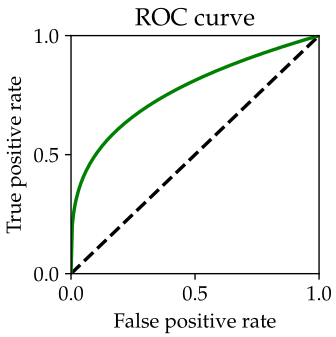
\includegraphics[width=0.5\linewidth]{image/roc.png}
        \caption{The ROC curve is plotted in the FPR–TPR plane.}
    \end{figure}
    \item Lemma 2 (Neyman–Pearson Lemma)
Suppose the likelihood functions $p(x \mid y)$ are continuous. Then the optimal probabilistic predictor that maximizes TPR subject to an upper bound on FPR is a deterministic likelihood ratio test.
\end{itemize}

\end{document}

